% This Source Code Form is subject to the terms of the Mozilla Public
% License, v. 2.0. If a copy of the MPL was not distributed with this
% file, You can obtain one at https://mozilla.org/MPL/2.0/.

\documentclass[a4paper,12pt]{article}
\usepackage[utf8]{inputenc}
\usepackage[russian]{babel}
\usepackage{amsmath, amssymb}
\usepackage[hyperfootnotes=false]{hyperref}
\usepackage{geometry}
\usepackage{indentfirst}
\usepackage{graphicx}
\usepackage{float}
\usepackage{enumitem}
\usepackage{caption}
\usepackage{tikz}
\usepackage{array}
\geometry{
	a4paper,
	top=24mm,
	bottom=30mm,
	left=20mm,
	right=20mm
}

\newcommand{\blfootnote}[1]{%
	\begingroup
	\renewcommand{\thefootnote}{}%
	\footnote{#1}%
	\addtocounter{footnote}{-1}%
	\endgroup
}

% Отступ первой строки абзаца 1 см
\setlength{\parindent}{1cm}
\setlength{\parskip}{0pt}
\linespread{1}                 % одинарный интервал

% Отключение нумерации страниц
\pagenumbering{gobble}

% Настройка подписей рисунков и таблиц
% Используем \caption* для отключения точки, но оставляем обычный \caption
\usepackage[labelsep=space, justification=centering]{caption}
\captionsetup[figure]{font=small}   % small = 11pt при 12pt основного шрифта
\captionsetup[table]{font=small}
\renewcommand{\figurename}{Рис.}
\renewcommand{\tablename}{Табл.}

% Убираем точку в конце подписи (переопределяем \caption)
\usepackage{etoolbox}
\makeatletter
\renewcommand{\fnum@figure}{\figurename~\thefigure}
\renewcommand{\fnum@table}{\tablename~\thetable}
\apptocmd{\@caption}{\def\@captionheadfont{\normalfont}\def\@captionfont{\normalfont}}{}{}
\makeatother

% Настройка списка литературы
\makeatletter
\renewcommand{\@biblabel}[1]{#1.}   % нумерация "1.", "2."
\makeatother

\begin{document}
	\begin{center}
		\subsubsection*{Курсовая работа по численным методам: }
		\subsubsection* {"Решение краевых задач для ОДУ второго порядка"}
		\subsubsection*{Выполнил студент третьего курса Физико-механического института, высшей школы ФФИ: Куликовских Илья}
		\subsubsection*{Группа: 5030302/30801}
		\subsubsection*{Преподаватель: Веселова Ирина Юрьевна}
	\end{center}
	
	\quad \textbf{Постановка задачи.} Используя интегро-интерполяционный метод , найти приближённое решение краевой задачи (выдаётся преподавателем) со вторым порядком аппроксимации уравнения и краевых условий на равномерной сетке. Исследовать зависимость погрешности решения от количества разбиений:
	
	\begin{equation}
		-\left[\dfrac{d}{dx} \left((4 - x) \dfrac{du}{dx}\right) - 2u\right] = \dfrac{10(x^2 -5x + 9)}{e^x}
	\end{equation}
	
	\quad С граничным условием: 
	
	\begin{equation}
		u \bigg|_{x=0} = 0, \quad u \bigg|_{x=2} = \dfrac{20}{e^2}
	\end{equation}
	
	\quad \textbf{Решение.} Построим уравнения аппроксимации краевой задачи в ДСК: 
	
	\begin{equation}
		-\displaystyle\int\limits_{x_i - \frac{h}{2}}^{x_i+\frac{h}{2}}  \left[\dfrac{d}{d\xi}\left(k(\xi) \dfrac{du}{d\xi}\right) -  q(\xi )u(\xi)\right]d\xi =\displaystyle\int\limits_{x_i - \frac{h}{2}}^{x_i+\frac{h}{2}} f(\xi)d\xi
	\end{equation}
	
	\begin{equation}
		\displaystyle\int\limits_{x_i - \frac{h}{2}}^{x_i+\frac{h}{2}} \dfrac{d}{d\xi}\left(k(\xi) \dfrac{du}{d\xi}\right)d\xi = k(\xi) \dfrac{du}{d\xi} \bigg|_{x_i - \frac{h}{2}}^{x_i + \frac{h}{2}} = k\left(x_i + \frac{h}{2}\right) \dfrac{u_{i+1} - u_i}{h} - k\left(x_i - \frac{h}{2}\right) \dfrac{u_i - u_{i-1}}{h}  
	\end{equation}
	
	\begin{equation}
			\displaystyle\int\limits_{x_i - \frac{h}{2}}^{x_i+\frac{h}{2}} q(\xi)u(\xi) d\xi = hq(x_i) u_i ,  \quad \displaystyle\int\limits_{x_i - \frac{h}{2}}^{x_i+\frac{h}{2}} f(\xi) d\xi = h f(x_i) 
	\end{equation}
	
	\quad Таким образом краевая задача (1)-(2) аппроксимируется системой линейных уравнений:
	
	\begin{equation}
		-\frac{k\!\left(x_i - \frac{h}{2}\right)}{h^2}\,u_{i-1}
		+ \left( \frac{k\!\left(x_i - \frac{h}{2}\right) + k\!\left(x_i + \frac{h}{2}\right)}{h^2} - q(x_i) \right) u_i
		- \frac{k\!\left(x_i + \frac{h}{2}\right)}{h^2}\,u_{i+1}
		= f(x_i),
	\end{equation}
	
	\begin{center}
		где $k(x) = 4 - x$, $q(x) = 2$, $f(x) = \dfrac{10(x^2 - 5x + 9)}{e^x}$.
	\end{center}
	
	\quad В итоге задача сводится к решению системы линейных уравнений:
	
	\begin{equation}
		A \mathbf{u} = \mathbf{b} \quad \Leftrightarrow \quad
		\begin{pmatrix}
			-\dfrac{k\!\left(x_i - \frac{h}{2}\right)}{h^2}
			& \dfrac{k\!\left(x_i - \frac{h}{2}\right) + k\!\left(x_i + \frac{h}{2}\right)}{h^2} - q(x_i)
			& -\dfrac{k\!\left(x_i + \frac{h}{2}\right)}{h^2}
		\end{pmatrix}
		\begin{pmatrix}
			u_{i-1} \\ u_i \\ u_{i+1}
		\end{pmatrix}
		= f(x_i).
	\end{equation}
	
	\begin{center}
		$\forall i \in [1, N-1]\cap\mathbb{N}$
	\end{center}
	
	\quad Прямое численное решение краевой задачи (1)-(2) имеет вид: 
	
	\begin{figure}[H]
		\centering
		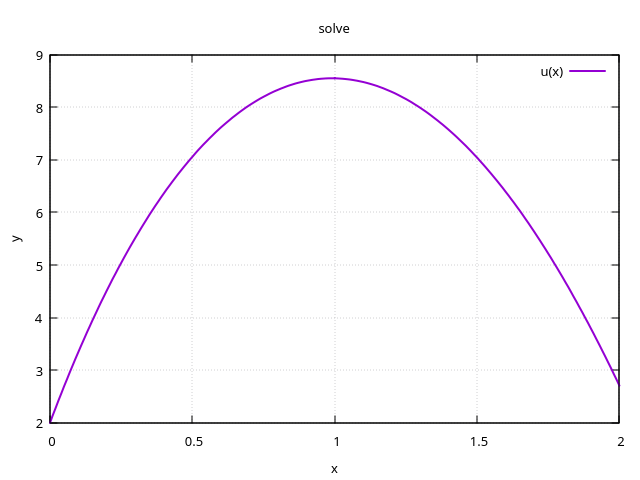
\includegraphics[width=0.8\textwidth]{solve.png}
		\caption{Численное решение краевой задачи}
		\label{fig:solve}
	\end{figure}
	
	\quad Построим зависимость чебышёвской номы погрешности от числа разбиений. Возьмём пробную функцию -- полином второго порядка $ u_{exact} = x^2 - x - 6$ и подставим уравнение (1) для определения явного вида правой части $f_{exact}(x)$:
	
	\begin{table}[H]
		\centering
		\caption{Зависимость чебышёвской нормы погрешности от числа разбиений (тест с нулевой погрешностью)}
		\label{tab:zero_error}
		\begin{tabular}{|c|c|c|c|}
			\hline
			$k$ & $N = N_0 \cdot 2^{k-1}$ & $\delta_k = max \{|u - u_{\text{exact}}|\}$ & $\delta_{k-1} / \delta_k$ \\
			\hline
			1 & 40   & $1.49 \cdot 10^{-13}$ & -- \\
			2 & 80   & $3.29 \cdot 10^{-13}$ & 0.45 \\
			3 & 160  & $7.06 \cdot 10^{-13}$ & 0.47 \\
			4 & 320  & $4.19 \cdot 10^{-12}$ & 0.17 \\
			\hline
		\end{tabular}
	\end{table}
	
\end{document}